\documentclass{jarticle}

\usepackage{graphicx}
\usepackage{listing,jlisting}
\usepackage{ascmac}
\usepackage{here}
\usepackage{txfonts}
\usepackage{listings, jlisting}
\renewcommand{\lstlistingname}{リスト}
\lstset{language=c,
	basicstyle=\ttfamily\scriptsize,
	commentstyle=\textit,
	classoffset=1,
	keywordstyle=\bfseries,
	frame=tRBl,
	framesep=5pt,
	showstringspaces=false,
	numbers=left,
	stepnumber=1,
	numberstyle=\tiny,
	tabsize=2
}

\begin{document}

\section{目的}
H8マイコンの割り込みについて理解を深め、割り込み制御をC言語で記述する方法を学ぶ。本実験では、発展的な課題として「UFOゲーム」作成に取り組み、キー入力処理と効果音処理を割り込みを用いて実現する。

\section{原理}
\subsection{UFOゲームの概要}
本実験の課題である「UFOゲーム」は、1980年代にゲーム電卓としてカシオ計算機から発売されたMG-880の「デジタルインベーダー」が元となっている。


「UFOゲーム」では、図1のようにキャラクタを使ってゲームフィールドを表現する。フィールドは、「:」によって分けられた照準フィールドと戦闘フィールドの2つから構成される。


照準フィールドには、敵を打ち落とすための数値が表示され、照準キーを押すたびに「...→0→1→2→...→8→9→n→0→...」のように順に変化する。戦闘フィールドには、フィールドの右側から左に向って敵が押し寄せてくる。押し寄せてくる速さは、ゲームが進行するにつれて徐々に速くなる。敵はインベーダを表す数字の0〜9と、UFOを示すnで表現されている。なお、インベーダは進行するたびに戦闘フィールドの右端に乱数で発生し、UFOは特定の条件下で発生する。


敵の撃墜は、照準フィールドの値を敵を示す値と一致させて発射キーを押すことで行われるが、戦闘フィールドに複数の同じ値をもつ敵が存在する場合には最も照準フィールド寄りの敵1つのみが撃墜される。


撃墜された敵は消滅し、撃墜された敵よりも照準側にある敵は右側へ退く。敵の左端が「:」まで到達したときに占領されて、ゲーム終了となる。ゲームの完成見本として、UFO\_game.motが後述の実験用のディレクトリにあるので、各自で検証すること。

\subsection{キー状態の判別}
今回の実験課題では、キーを押すごとに照準の値を順に変化させなければならないため、キー状態の判別は重要な処理となる。一般に、機械的な接点をもつスイッチの特性として、チャタリング現象が生じる。チャタリング現象は、接点が切り替え時に振動することによって生じ、短い時間(数msから数10ms程度)にONとOFFを繰り返す現象である。その値をそのままマイコンで取り込むと、図2のように、一度だけ押したはずが複数回押したように検出されるため、チャタリングの除去が必要となる。


チャタリングの除去にはハードウェア処理による手法とソフトウェア処理による方法があるが、実験ボードのようにキーがマトリクスで実装されている場合はハードウェア処理ではコストがかかるため、一般的にはソフトウェア処理で行われることが多い。


チャタリング処理のアルゴリズムの原理は単純で、入力信号履歴を参照して過去一定期間内の値が全て同じ時に、その値を参照時の値とするものである。一定期間内の値が全て一致しない場合はキー状態が遷移中であると考え、アプリ側で適切に処理する必要がある。

\subsection{リングバッファ}
キー状態の判別には一定期間内の信号履歴が必要となるため、キーをセンシングするたびに値を保存しておく必要がある。


リングバッファはこのような用途によく用いられ、図3のように、通常の配列のような一次元状のバッファの最初と最後をつなぎ合わせることでリング状のバッファを形成する。すなわち、リングバッファの大きさが過去の履歴を保存しておく大きさとなる.


リングバッファのどの位置に最新のデータが入っているかを示すためにポインタを用意し、データの更新を行うたびにポインタも更新する。このとき、リングバッファの実現に配列を利用する場合、ポインタの更新にあたっては配列の最後の次は配列の最初になることに留意しなければならない。このことは、過去の履歴の参照の際にも必要となるので注意すること。


\subsection{効果音の生成}
効果音を発生させる方法はいくつかあるが、ここでは単純な一定音程で一定の期間の音を生成する方法について考える。一定音程の単音を発生させる最も簡単な方法は、図4のように、矩形波を生成させる方法である。矩形波の生成は、一定期間ごとに出力値を変化させることで実現できる。


このとき、単音のみの生成に専念するのであれば一定期間をムダ時間ループで実現すればよいが、本課題では音を生成することによってゲームの進行を妨げることができない。このため、割り込みを音程の半周期ごとにかけることで出力値の変化のタイミングをはかることで、ムダ時間の弊害を取り除くように工夫する。


また、効果音の長さは音長を割り込みの間隔で割ることで、指定時間となる割り込みの回数を知ることで制御を行う。


なお、効果音生成用の割り込み間隔は音程によって変化するため、他のキー処理等の常に一定間隔の割り込みと共用することはできない。このため、効果音生成用に専用のタイマを準備して割り込み制御を行うことが必要である。


\section{使用機器}
使用機器を以下に示す。
\begin{enumerate}
\item H8マイコン
\item USBケーブル
\item パーソナルコンピュータ
\end{enumerate}

\section{実験方法}
本課題では、内蔵されているタイマ2つを割り込み発生源として使用する。タイマ0を効果音生成専用のタイマとして割り込み優先度をプライオリティ1(高優先度)として用いる。プライオリティ1の優先度を使用するためには、UIビットの設定が必要であり。USE\_UI();をプログラムの最初に実行する必要がある。また、タイマ0をプライオリティ1に設定するためには、更にtimer\_pri\_set(ch, pri)で設定を行う必要がある(ch:タイマのチャネル番号、pri:プライオリティ値)。割り込みハンドラはint\_imia0()であり、sound.c内に記述する。


タイマ1は常に一定間隔(1ms)で割り込みを発生し、キーのセンシング・敵の進行速度・時間待ち等の処理を行うものとする。割り込みハンドラはint\_imia1()であり、ufo.cに記述する。


課題にあたっては、/home/class/j3/jikken/kouki/no4以下に課題に必要なフアイルを置いてあるので、必ず全てのファイルを各自でコピーして利用すること。


\subsection{課題1 キー読み込みの実装}
コピーしたファイル(特に、ufo.c, key.c)をよく読み、key.cに記述されている各関数を完成させなさい。


key\_sense()はタイマ1の割り込みごとに呼び出され、リングバッファにキーマトリクスの列ごとのスキャンデータを格納するように作成すること。リングバッファはkey.cで大域変数として宣言されているkeybuf[p][r]であり、pは参照ポインタ、rは列を表すものとする。また、割り込み処理をまたぐリングバッファのポインタはkeybufdpを用いること。なお、キースキャンの方法等については、最後のページにある補足のキーマトリクスとセンシングを参照のこと。


key\_check(keynum)はチャタリング除去を行った結果を返す。その戻り値はkey.cで定義されているKEYOFF(指定キーは押されていない)、KEYON(指定キーが押されている)、KEYTRANS(指定キーは変化中)、KEYNONE(指定キーは存在しない)のいずれかを正しく返すものとする。また、チャタリング除去で参照するバッフア上の範囲は、key.cで定義されているKEYCHKCOUNTの長さとする。課題ができたら、必ずその時点でコンパイル・実行して動作を確認し、プログラムと動作のチェックを受けること。チェックを受けずに先の課題を行うことは認めない。


\subsection{課題2 効果音生成の実装}
コピーしたフアイル(特に、ufo.c, sound.c)をよく読み、sound.cに記述されている各関数を完成させなさい。


sound\_beep(hz、msec, vol)は引数(hz:音程周波数で単位は[Hz], sec:音長で単位は[ms], vol:振幅で矩形波のD/A上限値)から計算して、音程のための割り込み間隔・音長のための割り込み回数・短形波の振幅を求めて必要な記述を加えること。


sound.cで宣言されている大域変数timer0\_countは割り込み回数を格納し、play\_countは指定音長に対する割り込み回数を格納da\_ampは指定振幅を格納するように、それぞれ準備されている。-課題ができたら、必ずその時点でコンパイル・実行して動作を確認し、プログラムと動作のチェックを受けること、チェックを受けずに先の課題を行うことは認めない。


\subsection{課題3 UFOゲームの発展}
以下の課題に取り組み、UFOゲームを更に発展させる。細部の仕様は適宜定めてよいが、レポートに記述すること。
\subsubsection*{・課題3-1}
自機数を導入し、占領された場合と、発射キーを押したときに照準値と同じ値の敵がいない場合(攻撃に失敗した場合)に自機数が減るようにして、自機数が0になったときにゲームオーバとなるように変更する。
\subsubsection*{・課題3-2}
出現する敵数と発射できる弾数を制限し、敵を全部撃破したら面クリアとする。面が進むにつれて条件を厳しくし、占領されたときにゲームオーバとなるように変更する。


\section{実験結果}
\subsection{課題1 キー読み込みの実装}
key.hに宣言されている関数を実装することで、チャタリングを除去して、キーでゲームを操作することが可能になった。


ソースファイルをリスト1に、Makefileをリスト2にそれぞれ示す。

\subsection{課題2 効果音生成の実装}
sound.hに宣言されている関数を実装することで、ボタン操作に応じて効果音がなるようになった。


ソースファイルをリスト3に示す。Makefileは課題1のリスト2と同じである。

\subsection{課題3 UFOゲームの発展}
\subsubsection*{・課題3-1}
課題の条件を満たすプログラムを作成し、実際に動作することを確認した。


ソースファイルをリスト4に示す。Makefileは課題1のリスト2と同じである。

\subsubsection*{・課題3-2}
ステージが進むに連れて、敵の数は多くなり、余分な弾数が少なくなるようにした。敵または弾数が99以上の場合、表示は99のままで99未満になるとその数値が表示される仕様にした。表示中の「E:」は敵の残り、「B:」は残り弾数、そして「S:」は現在のステージを表す。


ソースファイルをリスト5に示す。Makefileは課題1のリスト2と同じである。


\section{検討課題}
\subsubsection*{・検討課題1}
ufo.cをよく読んで、どのようにして「今、キーが押された」かを検出しているかについて、説明しなさい。


1ループ前のキーの状態を保持し、現在のキーの状態と比較することにより実現されている。1ループ前に押されていない、かつ現在押されていればキーは今押されたことになる。

\subsubsection*{・検討課題2}
補足の図5キーマトリクス回路において、キースイッチと直列にダイオードが挿入されていないとどのような不具合が生ずるか、説明しなさい。


読み取ろうとしている行のいずれかのキーを押した状態で、そのキーと同じ列の他のキーを1つ以上に押すと、5V端子とGNDが短絡された状態になり、大きな電流が流れるため危険になる。

\subsubsection*{・検討課題3}
sound.cで実装したような割り込み処理による効果音生成において、効果音の音程が高くなると、どのような悪影響が生じてくるかについて検討せよ。


効果音のための割り込みの回数が多くなり、メインの処理、キーの処理に充てられる時間が減り、キーの取りこぼしが発生したり反応が遅くなったりして快適に遊べなくなる恐れが出てくる。

\newpage

\begin{figure}[h]
	\begin{center}
		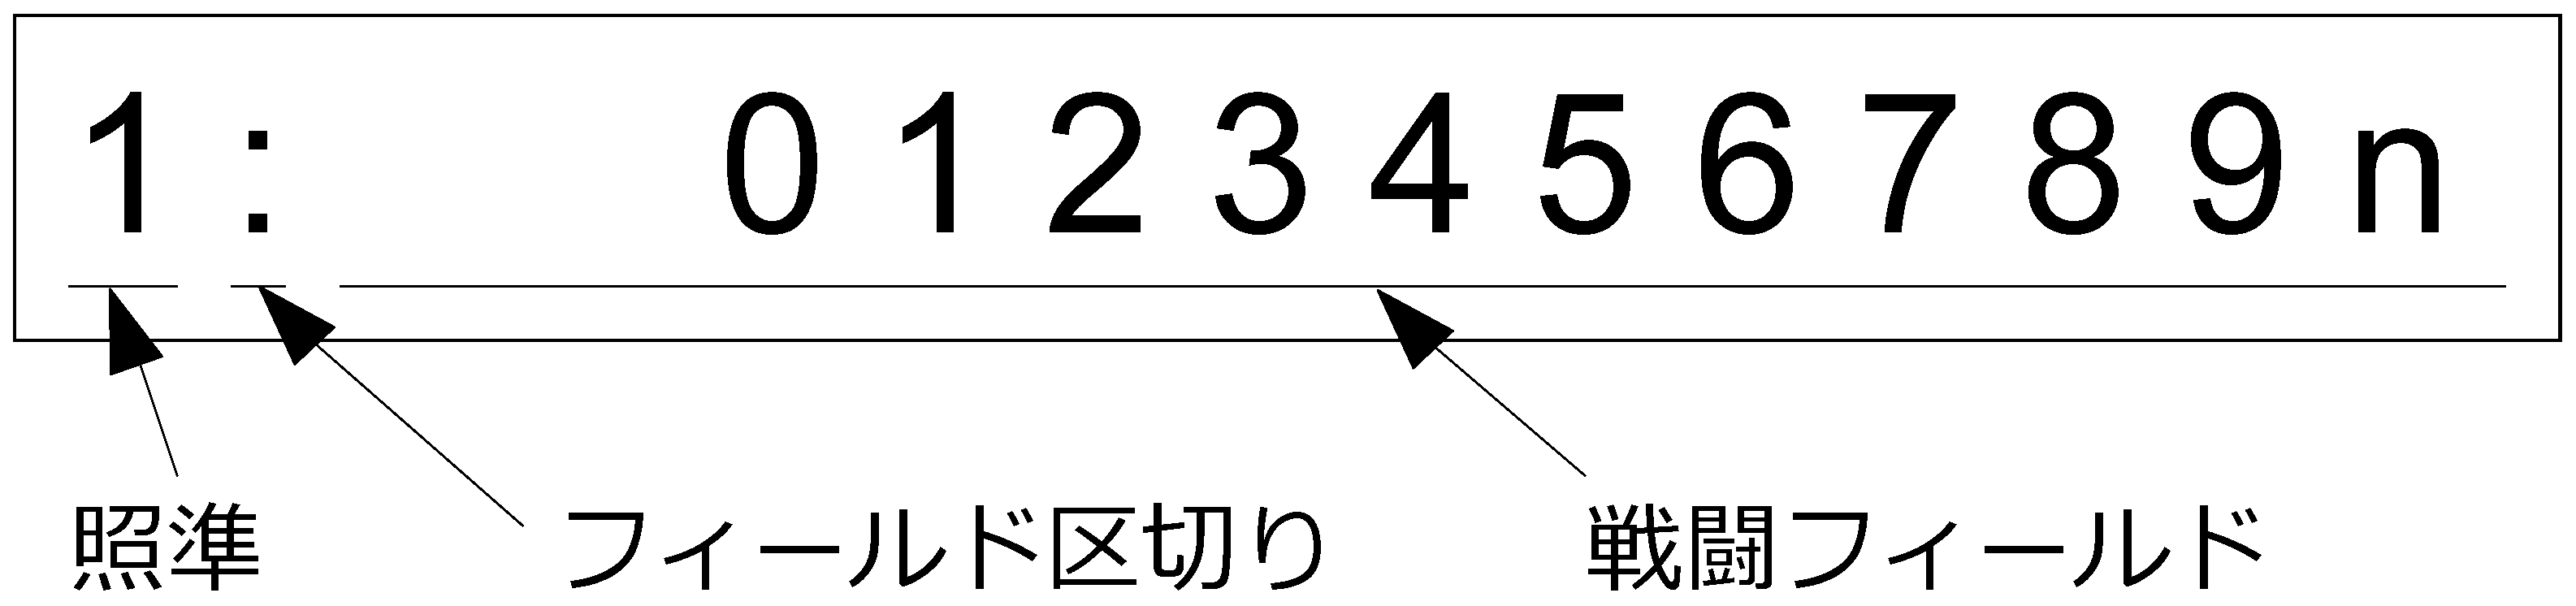
\includegraphics[width=10cm]{./figure1.eps}
	\end{center}
	\caption{UFOゲームのフィールド}
\end{figure}

\begin{figure}[h]
	\begin{center}
		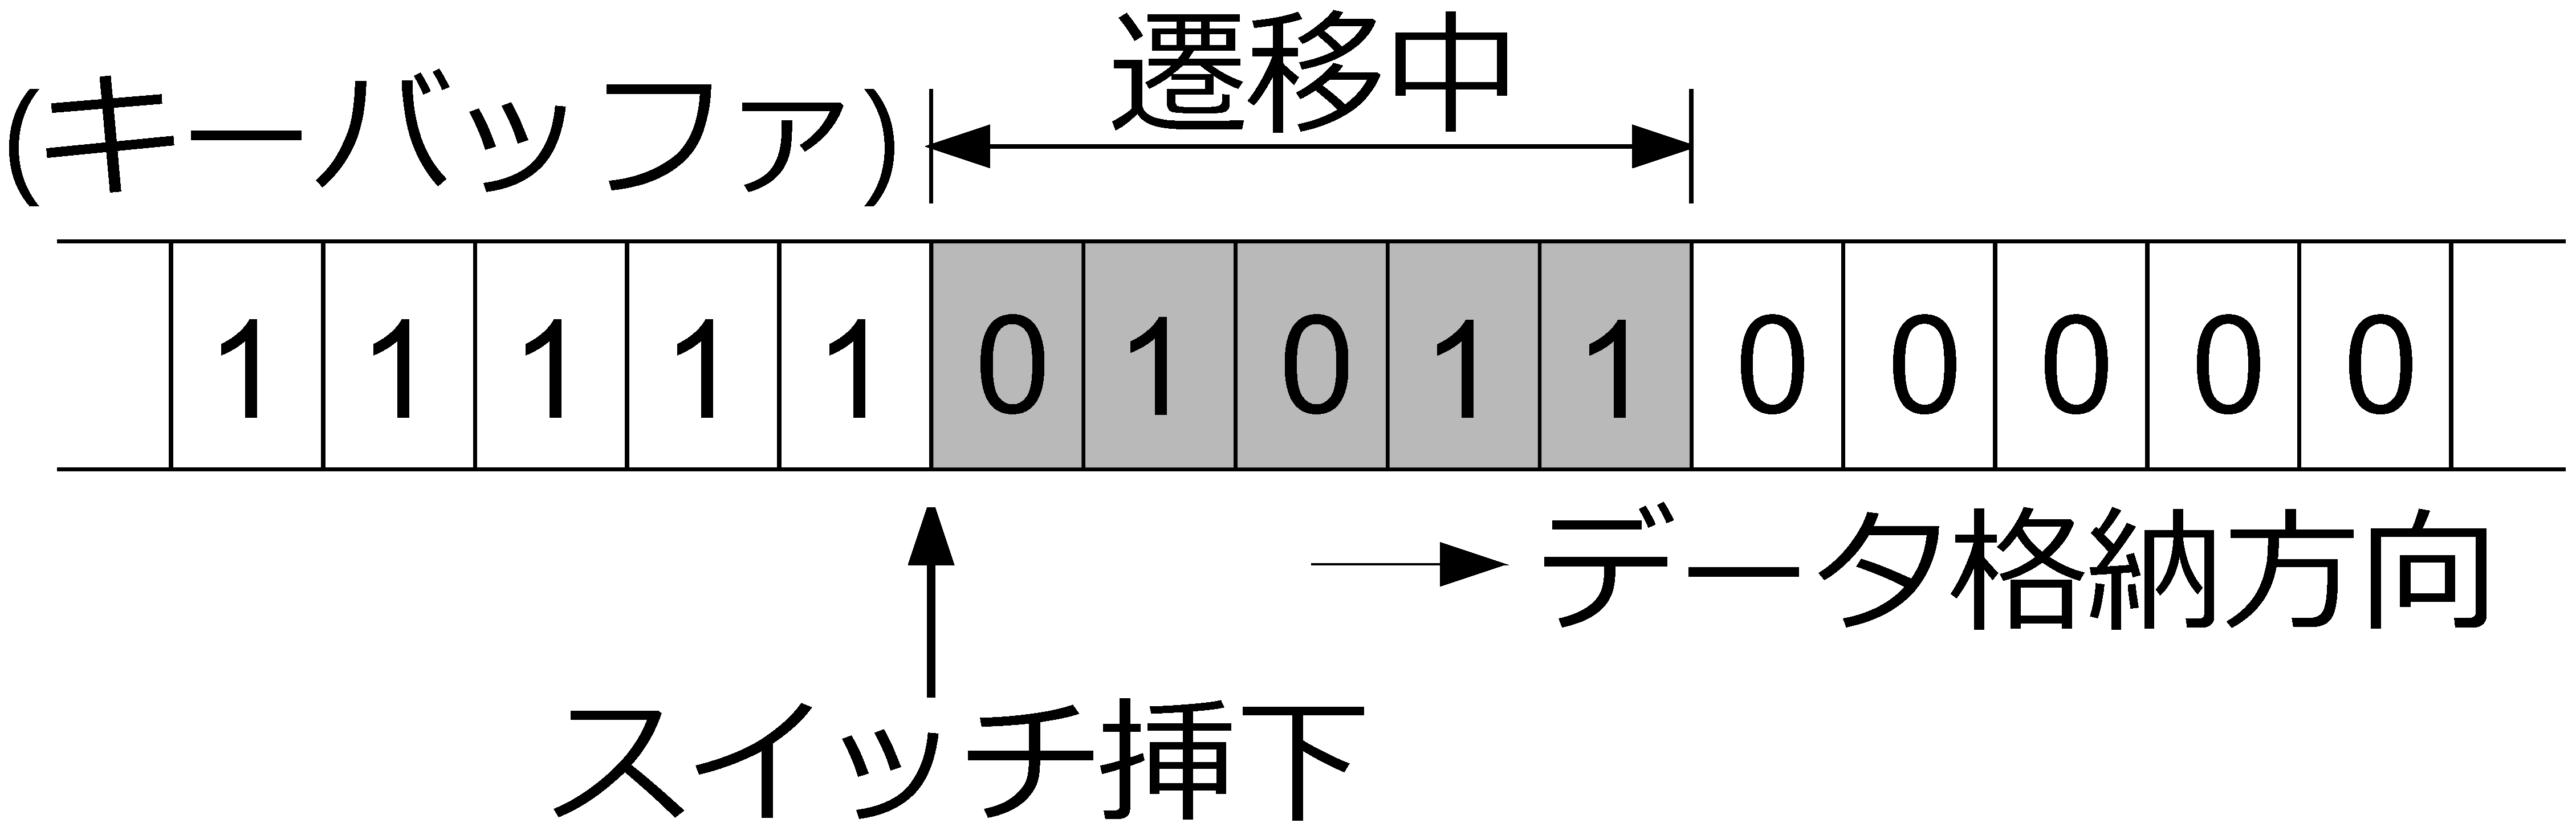
\includegraphics[width=10cm]{./figure2.eps}
	\end{center}
	\caption{チャタリング発生時のデータバッファの様子}
\end{figure}

\begin{figure}[!h]
	\begin{center}
		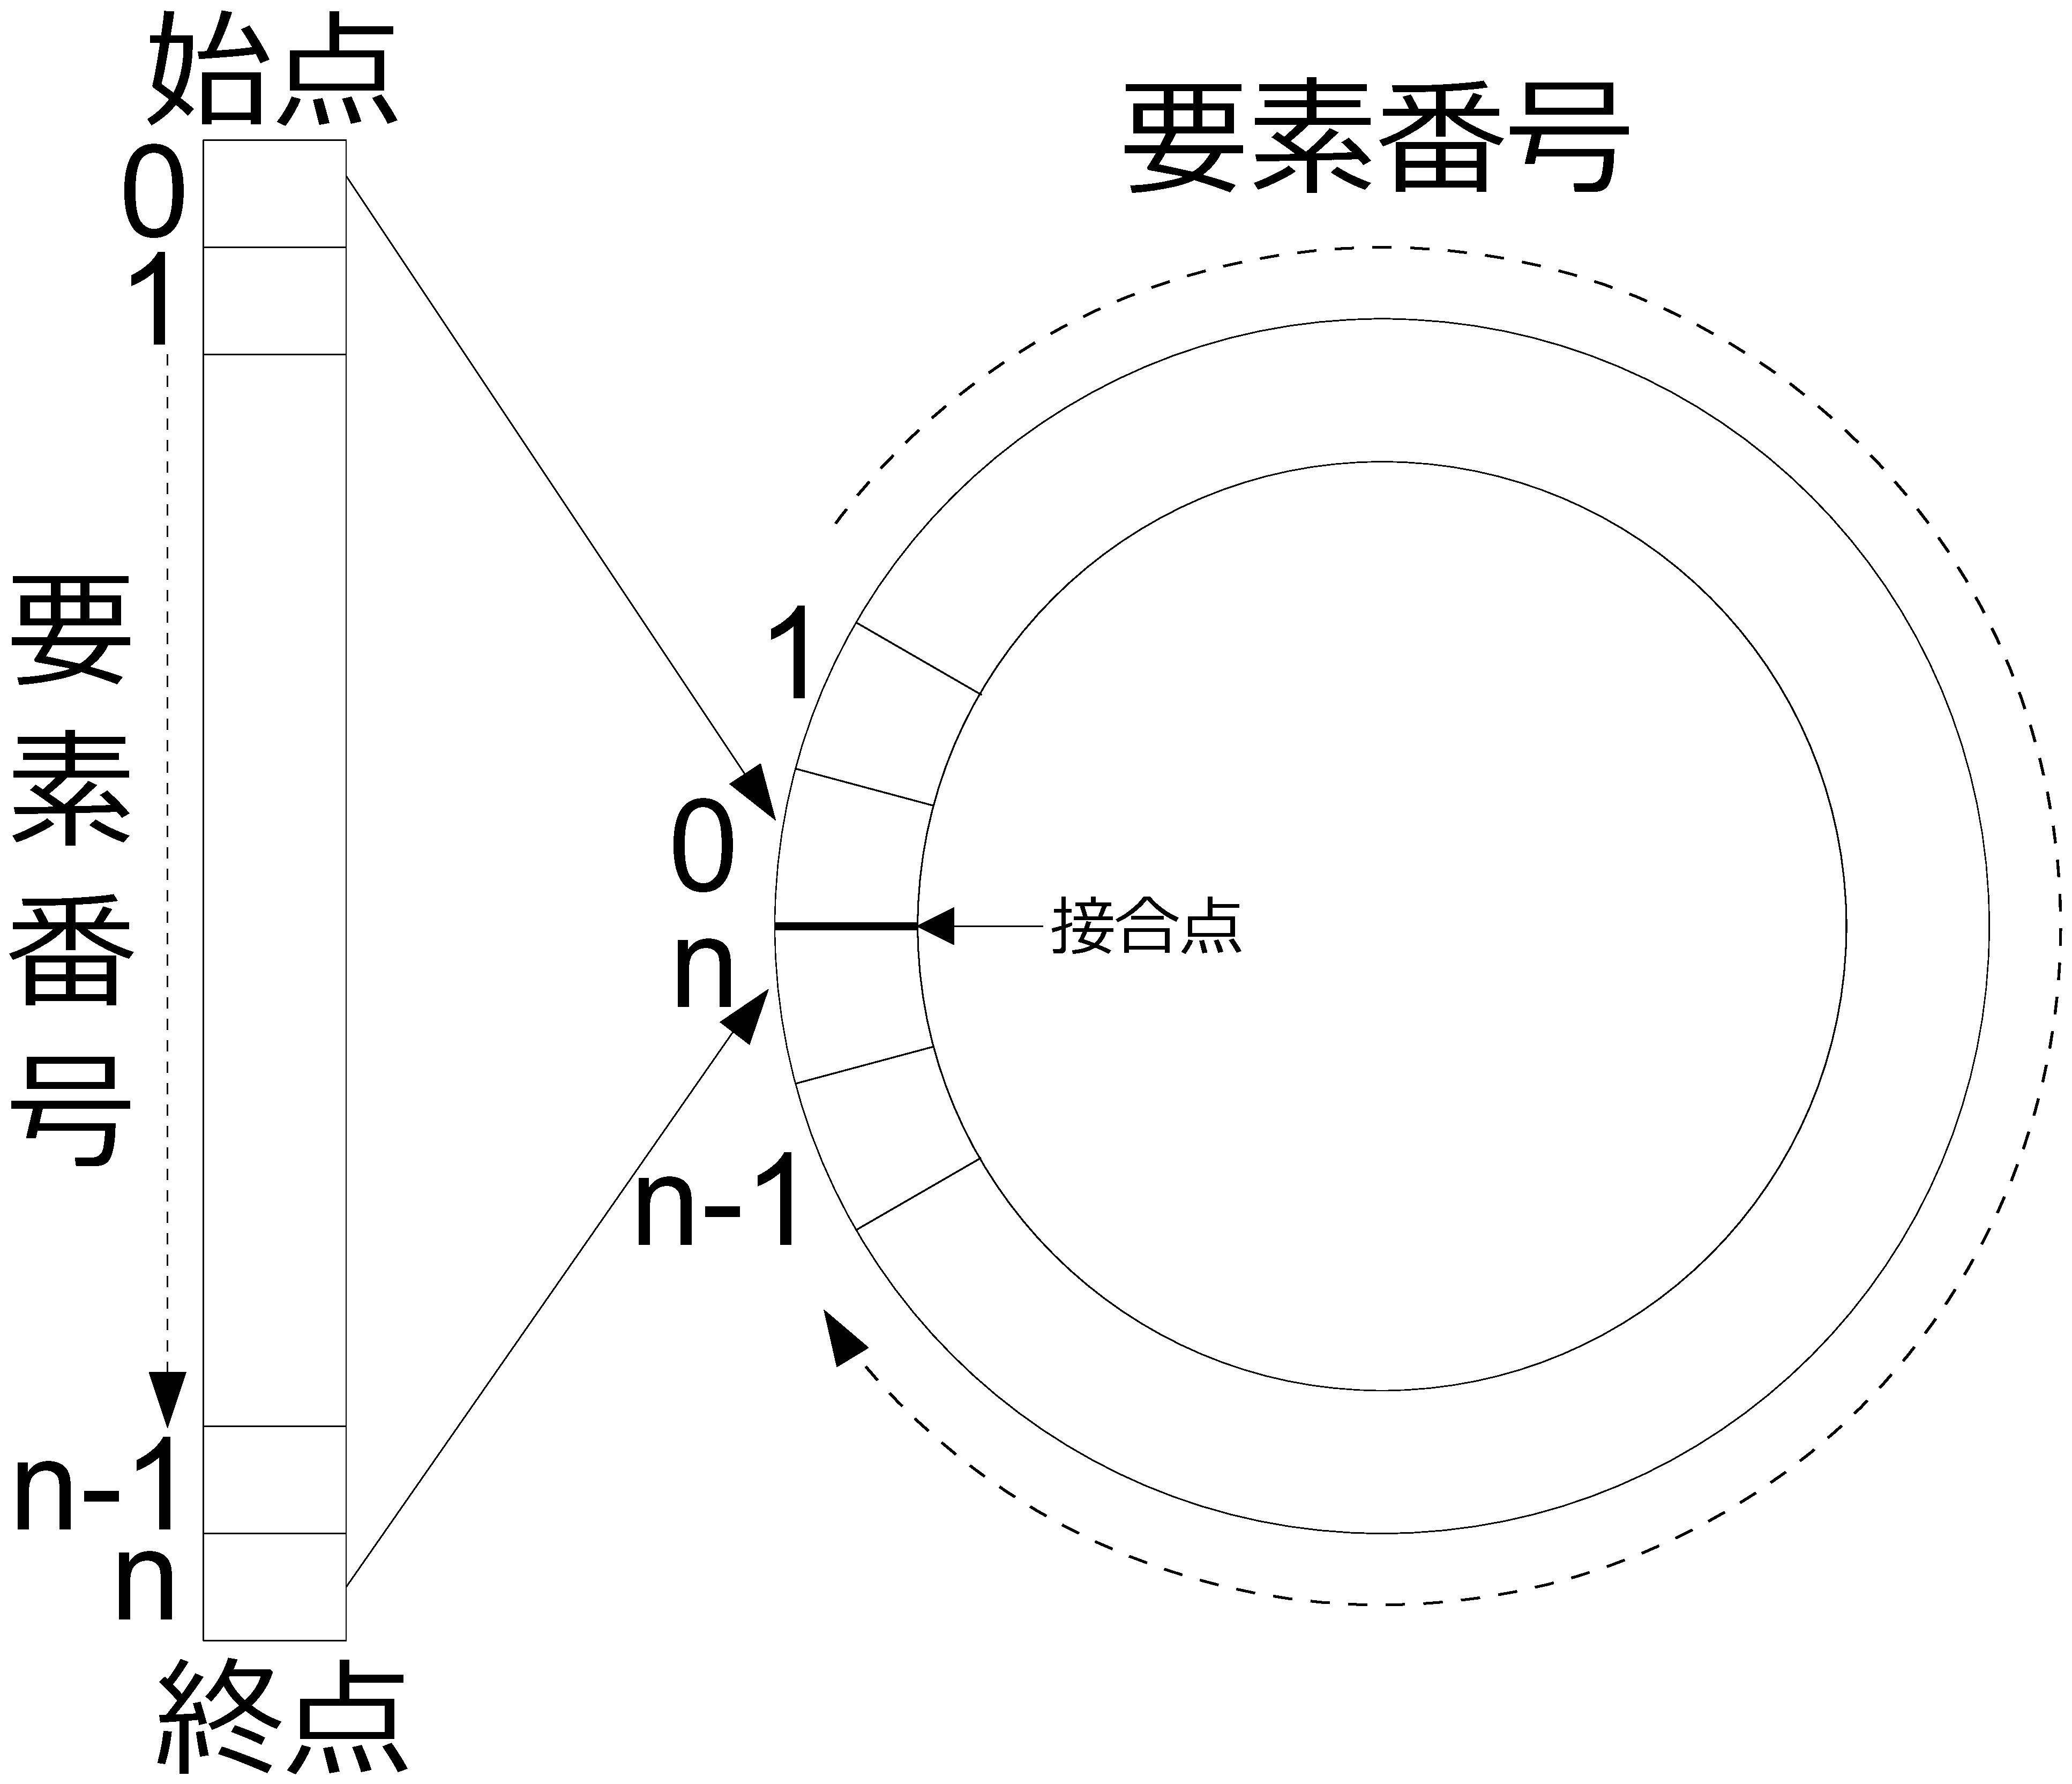
\includegraphics[width=10cm]{./figure3.eps}
	\end{center}
	\caption{リングバッファの構成}
\end{figure}

\begin{figure}[!h]
	\begin{center}
		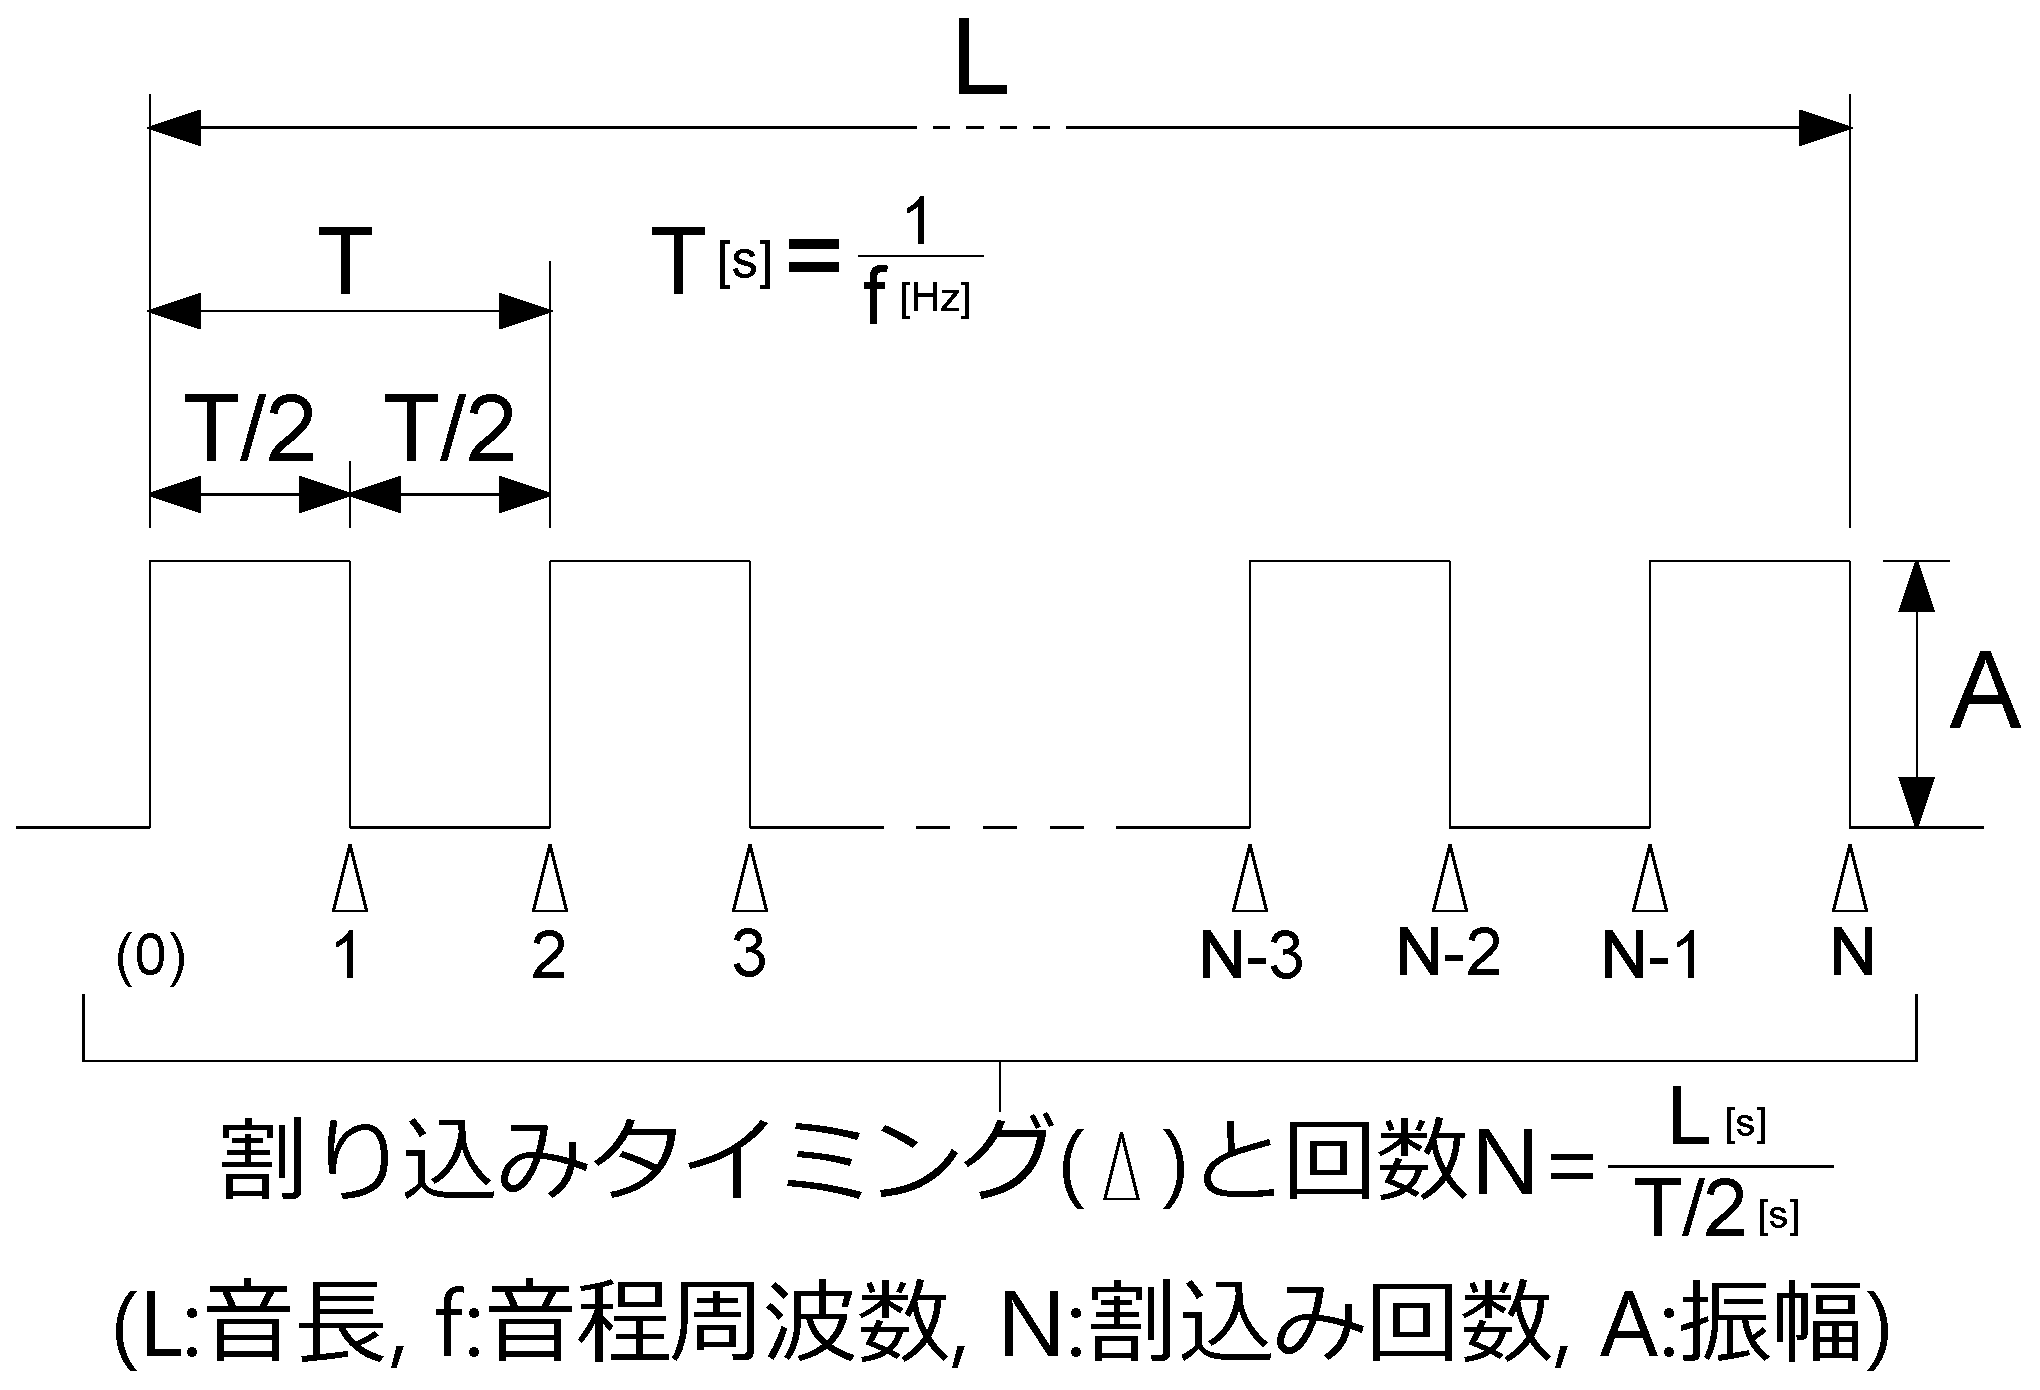
\includegraphics[width=10cm]{./figure4.eps}
	\end{center}
	\caption{効果音の波形}
\end{figure}

\newpage

\lstinputlisting[caption=key.c]{../key.c}
\lstinputlisting[caption=Makefile]{../make-ufo}
\lstinputlisting[caption=sound.c]{../sound.c}

\if0
\lstinputlisting[caption=課題3-1のufo.c]{../ufo31.c}
\lstinputlisting[caption=課題3-2のufo.c]{../ufo32.c}
\fi

\newpage

\begin{figure}[h]
	\begin{center}
		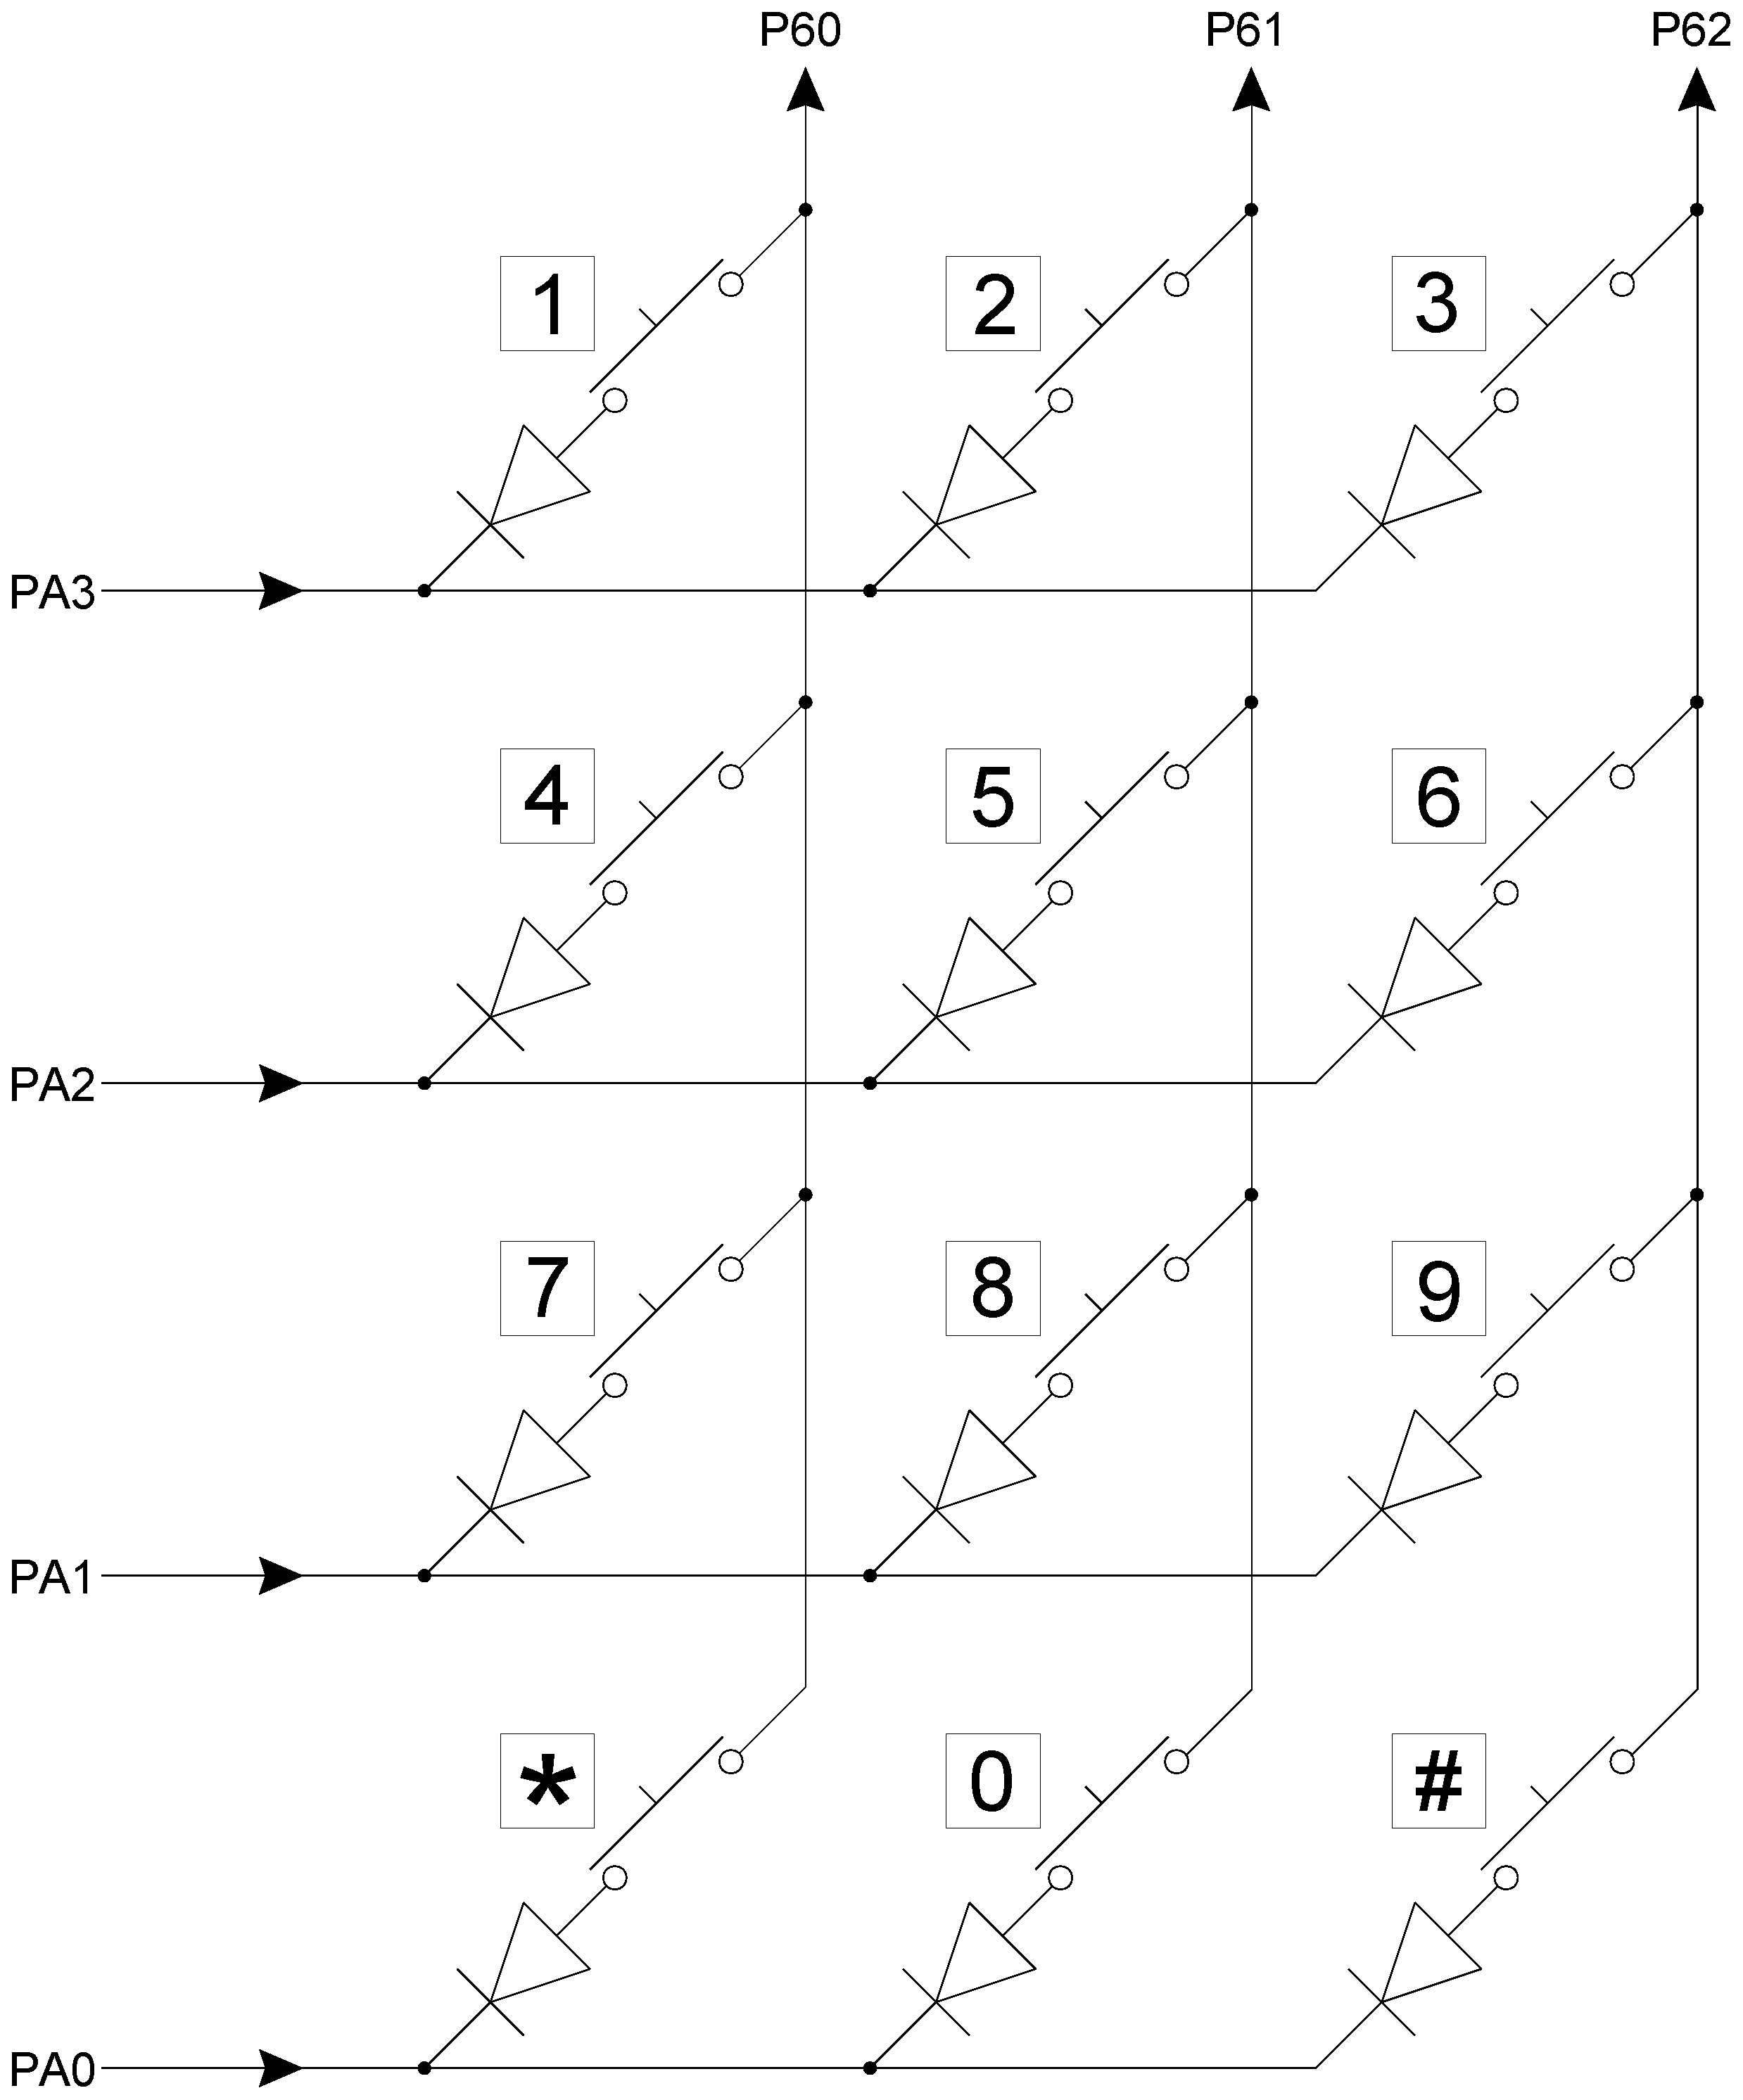
\includegraphics[width=10cm]{./figure5.eps}
	\end{center}
	\caption{キーマトリクス回路図}
\end{figure}


\end{document}

